\documentclass[11pt]{article}
\usepackage{pdfpages}
\usepackage{graphicx}
\usepackage{tikz}
\usepackage{hyperref}
%\usepackage{fancyref}

% usage: \fnurl{URL}{link text}
\newcommand\fnurl[2]{%
\href{#1}{#2}\footnote{\url{#1}}%
}


% Ignore page numbers for title page
\setcounter{page}{0}

\title{Explain Shell for Chrome \& ExplainShell Trends\\Final Report}
\author{}
\date{Fall 2014}

\begin{document}
% ----- Letter of Transmittal -------------------------------------------------
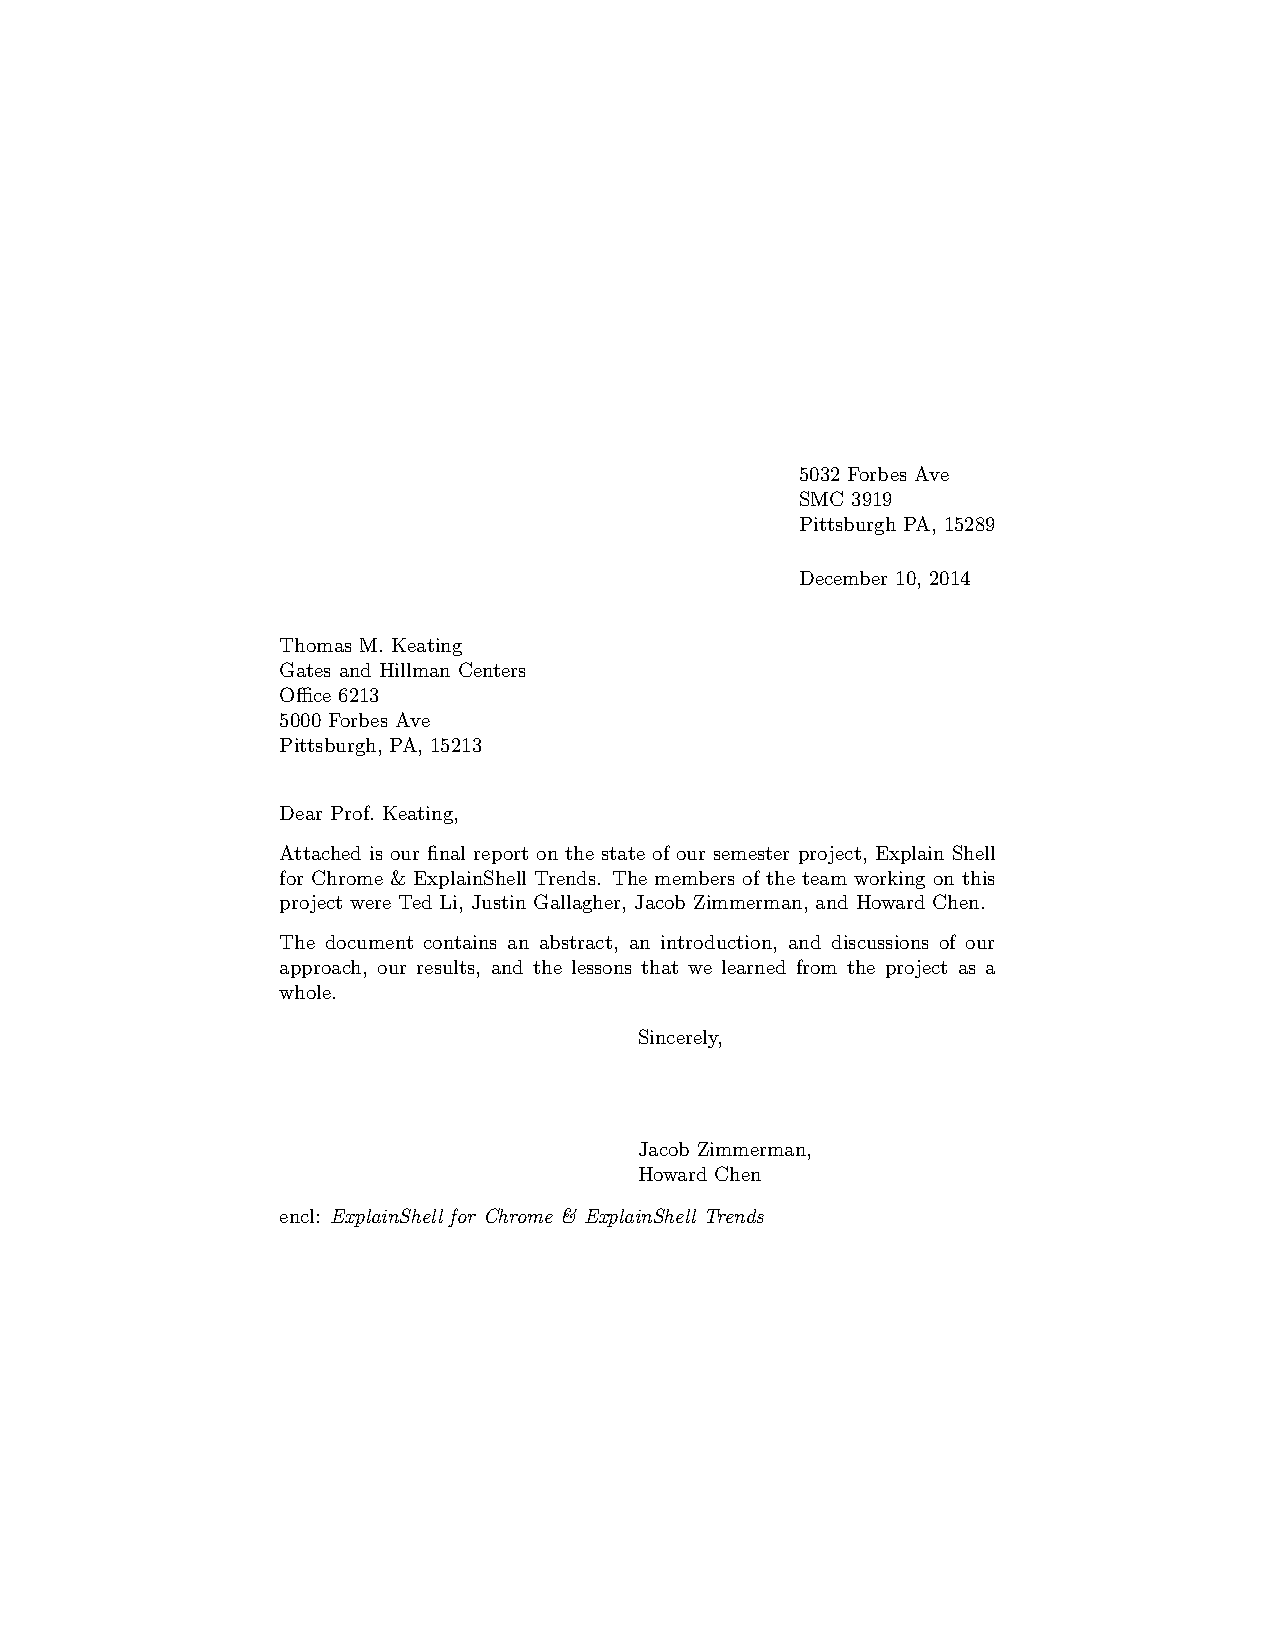
\includepdf{../letter/letter.pdf}

% ----- Title Pages -----------------------------------------------------------
\thispagestyle{empty}
\maketitle
\thispagestyle{empty}

\begin{center}
  \textit{Submitted to} \\
  Thomas M. Keating \\
  Assistant Teaching Professor \\
  School of Computer Science \\
  Carnegie Mellon University

  \mbox{} \\

  \textit{Prepared and submitted by} \\
  Jacob Zimmerman \\
  Howard Chen \\
  School of Computer Science \\
  Carnegie Mellon University

  \mbox{} \\
\end{center}

\begin{abstract}
  When working in a command line environment, running correct, safe shell
  commands is a daunting task---\texttt{man} pages and Google searches often
  don't cut it or take too much time. We solve this problem of educating people
  about various shell commands by wrapping access to a well-known website,
  ExplainShell.com, in a Chrome extension.  We also provide an accompanying
  website to aggregate data and provide a community around learning shell
  commands. The extension provides immediate access to the website so as to
  minimally detract from the user's current workflow. We implemented all the
  planned features, including processing the page to turn shell commands into
  clickable links as well as optionally displaying an informational popup in
  the context of the page. Meanwhile, the website is able to show community
  wide trends about how people are learning commands to help other get engaged,
  compounding the goals of our extension.
\end{abstract}

\newpage
% ----- Table of Contents -----------------------------------------------------
\pagenumbering{roman}

\tableofcontents

\newpage
% ----- Body ------------------------------------------------------------------
\pagenumbering{arabic}

\section{Introduction}

We discuss the circumstances warranting the need for our project, give an
overview of our project, and show how it solves the problems we outlined. We
also analyze the effectiveness of our Literature Review, as well as how well our
final accomplishments compare with our original goals.

\subsection{Background}

For those who work in a command line environment, it's hard to find references
that are both accurate and accessible when trying to run particular commands.
Manual pages certainly satisfy the ``accurate'' stipulation, as they're often
the most definitive source of information on a command. On the other hand,
Google has made vast amounts of accessible information, but it sometimes lacks
the high quality found in man pages.

By and large, users favor accessibility over accuracy, meaning that users copy
and paste commands and lines of code without considering their accuracy. This
poses a grave threat to users, as people risk running malicious or insecure
commands unknowingly.

Luckily, there exist sites like ExplainShell.com which aim to rectify this
situation to some extent. By copying and pasting commands into ExplainShell.com,
users can see information for a particular command and all flags used or
technologies used, giving credibility to the correctness of particular commands.
ExplainShell works well, but it provides one additional step on top of the
simple copy/paste operation that users would otherwise perform. Unfortunately,
this extra step is oftentimes one too many.

\subsection{Project Overview}

The primary goal of our project was to reduce the invasiveness of this step in
people's normal workflow. Using a Chrome Extension that users could install
with a single click, we would be able to provide access to the same information
that ExplainShell provided, but directly in the context of the page.

This access manifests itself in the extension in two settings. With the first
option enabled, all lines of code that look like shell commands are turned into
links. Instead of having to copy, change tabs, and paste, users can simply
click to access the information. The alternative option is to merely hover over
the relevant lines and have an inline popup display the relevant information.

A secondary goal of our project was to provide a sort of community for people
learning and using shell commands. We wanted to take advantage of the
information we would have access to, given a sizable install base of our Chrome
Extension. This project, called ExplainShell Trends, would tap into the
clicks or hovers sent to our Chrome extension and send them off to a
centralized analytics site. Here, we crunch the data to display trends such as
such as most popular commands and sites, most viewed articles, and more.

By aggregating data from all installations of our Chrome extension, we
effectively ``crowd-sourced'' educating people about shell commands. We created
a collective learning grounds that was both accessible and accurate.
Additionally, even people who don't have the ExplainShell for Chrome extension
installed can see what sorts of commands people view most commonly so that
everyone can learn new skills.

\subsection{Analysis of Literature Review}

The literature on this sort of subject was nearly non-existent. What
documentation there is on shell scripting is usually of poor quality and widely
varied. Additionally, it's normally a topic learned in the process of doing
something else; shell scripting is generally a means to an end rather than a
pursuit in and of itself. This vicious cycle means that finding literature for
our topic was a struggle.

Overcoming this, We did manage to find value in sites like BashOneliners.com
and LinuxCommand.org. BashOneliners.com is a site dedicated to the collection
and explanation of single-line Bash snippets. LinuxCommand.org is a tutorial
for explaining the shell to first-time users. Both of these sites possessed an
element of what we wanted to encapsulate in our project, but also failed at
either encouraging community involvement or were of poor craftsmanship. Using
them as a reference point, we were able to refine our product and aim to fill a
gap in the current app ecosystem.

Apart from these sites, we used various walkthroughs and tutorials to guide our
development process, with varying effectiveness. Some notable references we used
were \fnurl{http://cwbuecheler.com/web/tutorials/2013/node-express-mongo/}{this
guide} by Christopher Buecheler, and the
\fnurl{https://developer.chrome.com/extensions/samples\#search:contextmenus}%
{Chrome extension sample code}. These sites helped in the sense that they guided
our technical implementation, but did little as far as providing insight or
ideas into what could be accomplished or tweaked to solve our problem.

\subsection{Successes}

Considering the product that we were able to produce in the end, I would say
that we were successful at achieving both of our goals---provide a convenient
way to look up shell commands and create a centralized site for people to
observe shell scripting trends. We have a working Chrome extension that puts
ExplainShell's information as close as possible to the user's workflow. Our
trends site is able to aggregate many pieces of information collected by our
Chrome extension. While we don't have a huge number of people using the app
presently, with a little bit of marketing, there is no reason why it couldn't
be a practical solution for people in the large.

It is interesting to note that the way the Chrome extension works now is
different from the way any of us planned it initially. Along the way, we
realized that the time required to implement certain features would be
prohibitively high, so we dropped them, but because of the way we planned the
development of the extension (see Approach), nothing that we ended up having to
drop significantly affected our progress towards our original goals. We discuss
the difference between our original plans and final outcomes in more detail in
Approach and Results.

\section{Approach}

In this section, we outline the various phases of our development cycle. We make
special note of the technologies used to implement the extension and the site.

\subsection{Phase 1}

We planned Phase 1 of our project as the minimum viable product that could add
value on top of ExplainShell.com. For this phase, we implemented a Chrome
extension that allowed the user to select text, right click and be presented
with a context menu item directing the user directly to ExplainShell.com in a
new tab. We implemented this very shortly after our planning session to have a
working product.

While there was certainly room for improvement at this step, Phase 1 was
important for initializing the infrastructure of our project. Without having to
get too heavily invested into the brunt of the projects work, we were able to do
things like initialize a Git repository for the project, lay out the core files
to the Chrome extension (written in JavaScript), and push a working app all the
way through the Chrome Web Store.

\subsection{Phase 2}

For Phase 2, we implemented the first of the two options for how to interact
with our Chrome extension: finding bash command lines in the page and turning
them into clickable links. This turned out to be somewhat tricky, as without
doing a significant amount of text processing, it's hard to figure out what is a
line of bash code and what isn't.

To combat this, we looked for certain classes that tend to be present on blocks
of bash code, including the CSS class ``\texttt{lang-sh}'', which is added by the Google
PrettyPrint processor, a common library for adding color to code snippets. In
addition, we also interpreted code blocks whose line started with the text
\texttt{\$ }, as it is a common practice online to preface bash oneliners in
this way. Obviously, this can't possibly cover all cases, but in our experience
it is able to identify a large number of bash commands within web pages.

\subsection{Phase 3}

The principal goal of this phase was to implement the other major option:
displaying a popup when the user hovers over a line of bash code. This end
result of phase diverged the most from our original intentions of all the
phases.

Originally, we had planed to provide a new interface around the
information collected and returned by the underlying ExplainShell application.
This interface was to be more mobile friendly and also suitable to a
light-weight popup. This would have required modifying the actual ExplainShell
backend (written in Flask) and submitting a Pull Request to the original
ExplainShell project. Due to our teams' limited knowledge of Flask and the
complexities involved with getting acquainted to a foreign code base, this
turned out to not be a viable path.

Instead, we implemented a popup that displayed the actual ExplainShell.com page
for that line of code. As it turned out, this aligned more or less equally with
our original goal for the popup. It remains accessible, and is only slightly
more clunky that we initially intended. For users looking to have the least
resistance possible, it provides a quick way of bring up the relevant
ExplainShell.com information. The popup used Bootstrap to provide the popup
skeleton and animations, which was chosen for its ease of use and widespread
documentation.

\subsection{Phase 4}

``Phase 4'' was the term that we used to refer to the ExplainShell Trends site
during project planning and development. Since this phase actually was a project
own its own for the most part, we were able to proceed on development in this
phase alongside development of the Chrome extension.

We implemented the Trends site as a Node.js application with a MongoDB backend.
This was the best option because as a team, we were most familiar with Node.js,
and MongoDB's schema-less approach to data storage allowed our models to develop
rapidly as we adjusted the trends site and added features to it. The visible
portion of the trends site was implemented again using Bootstrap with a library
for incorporating JSON-based tables into the page.

The trends site is capable of querying information based on most recently
clicked items, top sites, and top articles. The trends site frontend is capable
of taking any of these returned datasets and sorting them by any field. All in
all, these endpoints provide a wide perspective of what sort of commands are
popular or potentially interesting to command line users.

\section{Results}

Our ExplainShell for Chrome and ExplainShell Trends projects are both successful
when evaluated in terms of our proposed evaluation criteria. Both ExplainShell
for Chrome and ExplainShell Trends are user-friendly and informative, bridging
the gap between accessibility and accuracy of information. Each embodies a
solution that helps people learn new things about command line shell code,
improving on the solutions that already exist. Additionally, the Chrome
extension lowers the barriers to looking up information about a command before
running it, meaning that users are safer from malicious attacks.

At the end of our project, we were able to implement all but three of the
milestones on our revised Gantt chart, all of which related to the public
ExplainShell API. As discussed earlier in the subsection on Phase 3, even though
we were not able to successfully contribute to ExplainShell's Flask backend,
progress towards our original goals and design for the extension didn't entirely
falter.

We had initially allocated time for contributing a public API to
ExplainShell for the purpose of making a responsive inline popup for when a user
would hover over or tap on a line of shell code. However, realizing that the
time required to implement this feature was prohibitively high, we managed to
find a different solution to provide the user with a simple popup by just
embedding the relevant ExplainShell page itself in the popup.

We have included our project's Gantt chart and revised Gantt chart in
Figure~\ref{gantt-revised} for reference (rotated for space considerations). The
second, third, and fourth items of the revised Gantt chart correspond to the
items we dropped.

\begin{center}
  \begin{figure}[h!]
    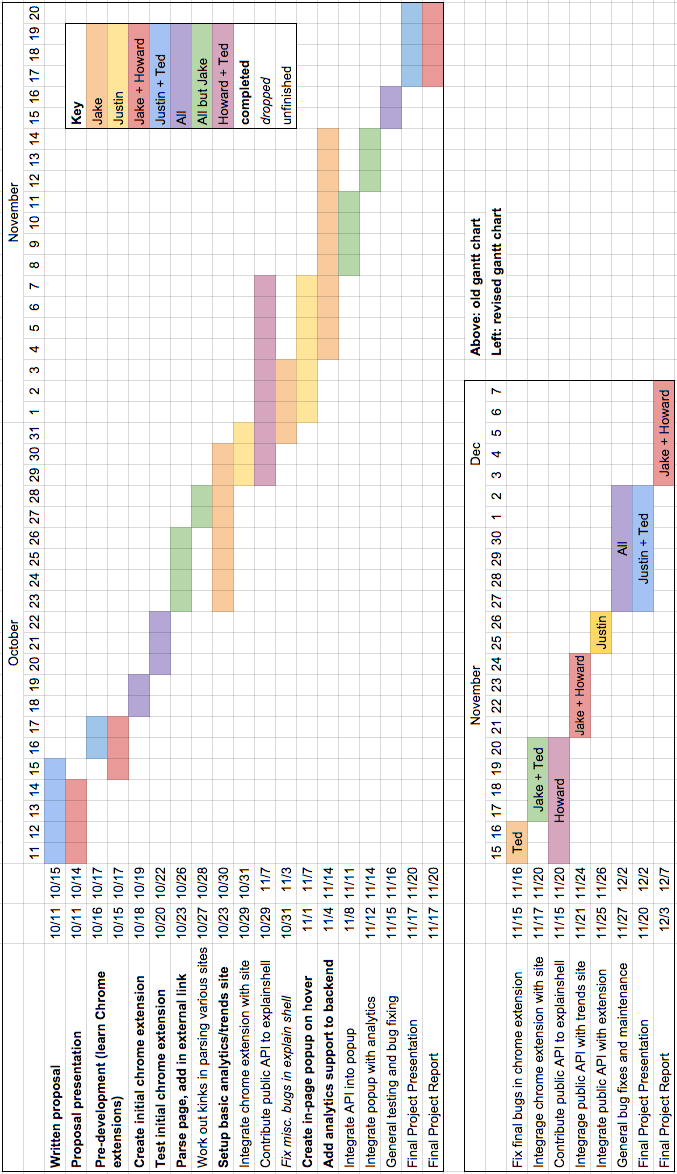
\includegraphics[height=0.95\textheight, keepaspectratio]{../../gantt-chart-revised-rotated}
    \label{gantt-revised}
    \caption{Revised Gantt chart, in context with progress on old Gantt chart}
  \end{figure}
\end{center}

\section{Discussions}

\subsection{Lessons Learned}

Our team learned a great deal from working on this project. Early on, we fell
embarrassingly behind schedule. Very little work had been contributed to the
project, and we were having trouble communicating between group members. Why
this ended up being the case is still somewhat mysterious, but we all recognized
that the lack of communication was hindering us.

Around the time we had to start doing weekly progress reports, we realized that
not nearly enough work was being accomplished. Jake had managed to pull together
a working implementation of Phase 1, but no other work had been done. The
turning point was that we had a meeting where we sat down and addressed the
lack of ownership and communication between team members---basically, we needed
to get our acts together and we all knew it.

Coming out of this meeting, we started to get some actual work done. We worked
diligently to make up time lost, checking items off our Gantt chart with renewed
vigor. It was a really powerful experience, seeing what can be accomplished with
just a little bit of discussion and understanding, and is what we all agree is
the most impactful lesson learned from the project.

As a team, we also learned many individual, technical lessons. For example,
Howard took the opportunity to learn how to use Git effectively to
collaborate on a programming project. Each member had the chance the learn new
things about web development and software engineering along the way.

\subsection{Recommendations}

If we were to do it over again, the principal recommendation we would adhere to
is to start earlier. Procrastinating on deadlines was one of the biggest
detriments to our productivity, and is ultimately what held us back from
contributing a public ExplainShell API back to the original project. Had we
managed our time effectively, we could have gotten ahead of the planned
schedule, ultimately yielding the necessary extra time to implement all the
features we had originally intended.

Another recommendation that we have is to understand the importance of
bottlenecks. When working on this project, we didn't accurately recognize which
steps of our project would require the most work. With two days of planning
compared with 2 hours of planning to come up with our Gantt chart, we could have
more adequately recognized these gaps in our planning and compensated for them
up front.

\newpage
% ----- References ------------------------------------------------------------

\begin{thebibliography}{9}
  \bibitem{explainshell}
      ExplainShell, \url{http://explainshell.com/}
  \bibitem{bashoneliners}
    Bash Oneliners, \url{http://www.bashoneliners.com/}
  \bibitem{linuxcommand}
    Linux Command, \url{http://linuxcommand.org/}
  \bibitem{chrome}
    Chrome extension context menu sample code,
    \url{https://developer.chrome.com/extensions/samples#search:contextmenus}
  \bibitem{chrome}
    Tutorial - Getting Started With Node.js, Express, MongoDB,
    \url{http://cwbuecheler.com/web/tutorials/2013/node-express-mongo/}
\end{thebibliography}

\end{document}
